\documentclass[conference]{IEEEtran}
\usepackage{cite}
\usepackage{amsmath,amssymb,amsfonts}
\usepackage{algorithmic}
\usepackage{graphicx}
\usepackage{textcomp}
\usepackage{xcolor}
\usepackage{booktabs}
\usepackage{url}
\def\BibTeX{{\rm B\kern-.05em{\sc i\kern-.025em b}\kern-.08em
    T\kern-.1667em\lower.7ex\hbox{E}\kern-.125emX}}

\begin{document}

\title{CALM\@: Calibrated, Order-Invariant, Label-Efficient Medical Question Answering with Small Language Models on a Two-GPU Budget}

\author{
\IEEEauthorblockN{Sabarna Saha}
\IEEEauthorblockA{\textit{Dept.\ of Power Engineering} \\
\textit{Jadavpur University}\\
Kolkata, India \\
sabarna.saha1308@gmail.com}
\and
\IEEEauthorblockN{Ankush Sil Sarma}
\IEEEauthorblockA{\textit{AI Engineer} \\
\textit{ZS Associates}\\
Pune, India \\
ankushsil17@gmail.com}
\and
\IEEEauthorblockN{Pawan Kumar Singh}
\IEEEauthorblockA{\textit{Dept.\ of Information Technology} \\
\textit{Jadavpur University}\\
Kolkata, India \\
pawansingh.ju@gmail.com}
}

\maketitle

\begin{abstract}
We work under a hard cap: two Kaggle T4 GPUs (16\,GB each), a few thousand labels, and a 4-bit base with LoRA adapters. CALM is what we fit inside it. The pipeline is deliberately ordinary---QLoRA on a small seed set, one temperature for calibration, a confidence threshold for abstention---and a Qwen2.5-7B student trained on 2{,}000 MedQA-USMLE labels lands at 0.633 test accuracy (95\% CI [0.606, 0.660]). That one temperature drops ECE from 0.086 to 0.026, and the most confident half of the test set is right 80.8\% of the time. The harder question was how to gain accuracy without paying in labels or training. Averaging the calibrated prediction over the four cyclic orderings of the options does it: accuracy rises to 0.655 (paired $+0.022$, 95\% CI $[+0.006,+0.038]$) and risk--coverage improves, for four forward passes and no decoding. Stripping out an option-ID prior, the obvious alternative, does not---the prior is essentially uniform here, so there is nothing to subtract, and the win is variance reduction rather than debiasing. Two more ideas helped less than we hoped. Routing only the least-confident items to a reasoning pass beats the fast reader by a small but significant margin, at about two extra tokens per question; a reflect adapter we trained for that job did no better than the student's own reasoning. Two did not work at all: teacher-guided self-distillation never helped validation accuracy, and on a matched 134-item subset five-sample self-consistency lost to a single calibrated pass. After several attempts, the configuration we kept was simple: a strong base model, limited supervision, calibration, abstention, and averaging across option orders.
\end{abstract}

\begin{IEEEkeywords}
medical question answering, calibration, selective prediction, selection bias, adaptive computation, parameter-efficient fine-tuning, resource-constrained learning
\end{IEEEkeywords}

\section{Introduction}
One question in MedQA-USMLE may contain a patient's age, several symptoms, lab panel, and a treatment history in the stem, and ask for one of the four possible options~\cite{medqa}. Large language models solve this problem easily. GPT-4 achieves high eighties~\cite{gpt4med}, Med-PaLM~2 reaches mid eighties~\cite{medpalm}. Compact 7--8B specialized models like Meerkat~\cite{meerkat} and MedMobile~\cite{medmobile} get above 60\%, but require large reasoning dataset and a lot of MedQA-USMLE labels for training. All of the above is impossible within the constraints of the Kaggle T4 GPU session with two 16\,GB GPUs.

We kept the budget constraint deliberately. The goal was not to top the leaderboard, but to see what still works when the hardware limit is real. We also cared whether the model knew when it was uncertain: accuracy alone hides two things a clinician would ask first---does the confidence mean anything, and can the model decline a question it is likely to miss~\cite{trustsurvey}? We track accuracy, calibration, and abstention quality together, and treat the last two as first-class.

Starting from the supervised QLoRA adaptation of a student model, we asked what cheap, post-hoc improvements actually help. There are two of them. Calibration with a single temperature parameter makes confidence meaningful and enables the working abstention rule. Order-invariant readout that computes the average of the predictions in four cyclic orders of options unexpectedly brings more than two points to the accuracy. There are also two other ideas that help a little or not at all, and we say this clearly: routing of the least-confident questions to a reasoning pass brings a small and significant improvement, but the teacher-guided self-distillation stage and the dedicated reasoning adapter do not.

Our contributions are as follows.
\begin{itemize}
\item \textbf{CALM}: a reproducible small-budget study of medical QA on two T4 GPUs, with 3B and 7B QLoRA students.
\item A \textbf{calibration-and-abstention layer} that reduces test ECE to 0.026 for the 7B student and enables risk--coverage analysis, in which the most confident 50\% of test items are answered with 0.808 accuracy.
\item An \textbf{order-invariant readout} that marginalizes over four cyclic option orders and raises test accuracy from 0.633 to 0.655 (paired 95\% CI $[+0.006,+0.038]$) and reduces AURC at four forward passes and no decoding. We show that the benefit is not option-ID debiasing---the prior is near-uniform and its removal (PriDe) does nothing---but reduction of order-dependent variance.
\item A \textbf{reflective routing} study of adaptive computation: routing the least-confident $\approx$2\% of items to a reasoning pass improves performance significantly at $\approx$2 extra decoded tokens per question, while a trained reflect adapter does not beat the reasoning of the base student (a negative result).
\item Two things we expected to help but that did not: teacher-guided self-distillation gives no validation gain, and self-consistency loses to a single calibrated pass while decoding far more.
\end{itemize}

\section{Related Work}
\textbf{Medical QA with language models.} Jin et al.\ created MedQA from medical licensing exams and posed the task as a canonical benchmark~\cite{medqa}. General purpose large models can solve it effectively with prompting~\cite{gpt4med,medpalm}, while a sequence of compact experts---Meerkat~\cite{meerkat}, MedMobile~\cite{medmobile}, and the HuatuoGPT-o1 reasoning models~\cite{huatuo}---has closed the performance gap using reasoning traces. We utilize the HuatuoGPT-o1-7B model as a teacher without any comparable training cost.

\textbf{Self-training.} Hinton et al.\ formulated the problem of soft-target transfer~\cite{hinton}; STaR~\cite{star} and self-consistency~\cite{selfconsistency} demonstrated how generated reasoning can enable smaller models to bootstrap themselves. The workhorse of semi-supervised learning is thresholding-confidence-based pseudo-labeling~\cite{pseudolabel}. We initially expected this stage to matter more; in our experiments the extra labels simply were not useful under the small-budget setting.

\textbf{Parameter-efficient adaptation.} LoRA and its quantized version QLoRA allow fine-tuning a 7B model in a single 16\,GB card~\cite{lora,qlora}; that makes everything we do possible within just two T4 GPUs.

\textbf{Calibration and abstention.} Guo et al.\ established that modern networks are typically miscalibrated and that temperature scaling is a simple yet powerful solution to this problem~\cite{guocal}. Selective prediction---predict an answer if a network is confident, abstain from doing so otherwise---is evaluated via risk--coverage plots and the area under them~\cite{selectivenet}. There is an emerging line of research arguing that being able to tell when to abstain is just as important as accuracy for clinical applications~\cite{abstain,trustsurvey}.

\textbf{Selection bias and option order.} Multiple choice tasks are subject to selection bias: a network can switch its answer depending on a particular option ordering~\cite{robustmcq,permbias}. PriDe explains much of that behavior with an option ID prior and attempts to remove this prior at inference time~\cite{robustmcq}. We found out that a calibrated student network does not have any significant option ID prior; however, the averaging of predictions over all permutations helps because it removes the order-sensitive variability of predictions.

\textbf{Reinforcement for small models.} Group Relative Policy Optimization~\cite{grpo} is commonly used as a post-training stage. However, according to recent studies, it has given uneven gains for small models under sparse rewards~\cite{smallrl}. Our findings are consistent with that picture.
\section{CALM Framework}
Figure~\ref{fig:arch} illustrates the architecture of the trained pipeline end to end. We introduce each component in turn; in Section~\ref{sec:results}, we discuss the selection of components according to our measurements, and provide two additional evaluation methods that require no further training of the network (order-invariant marginalization and reflective routing).

\begin{figure*}[t]
\centering
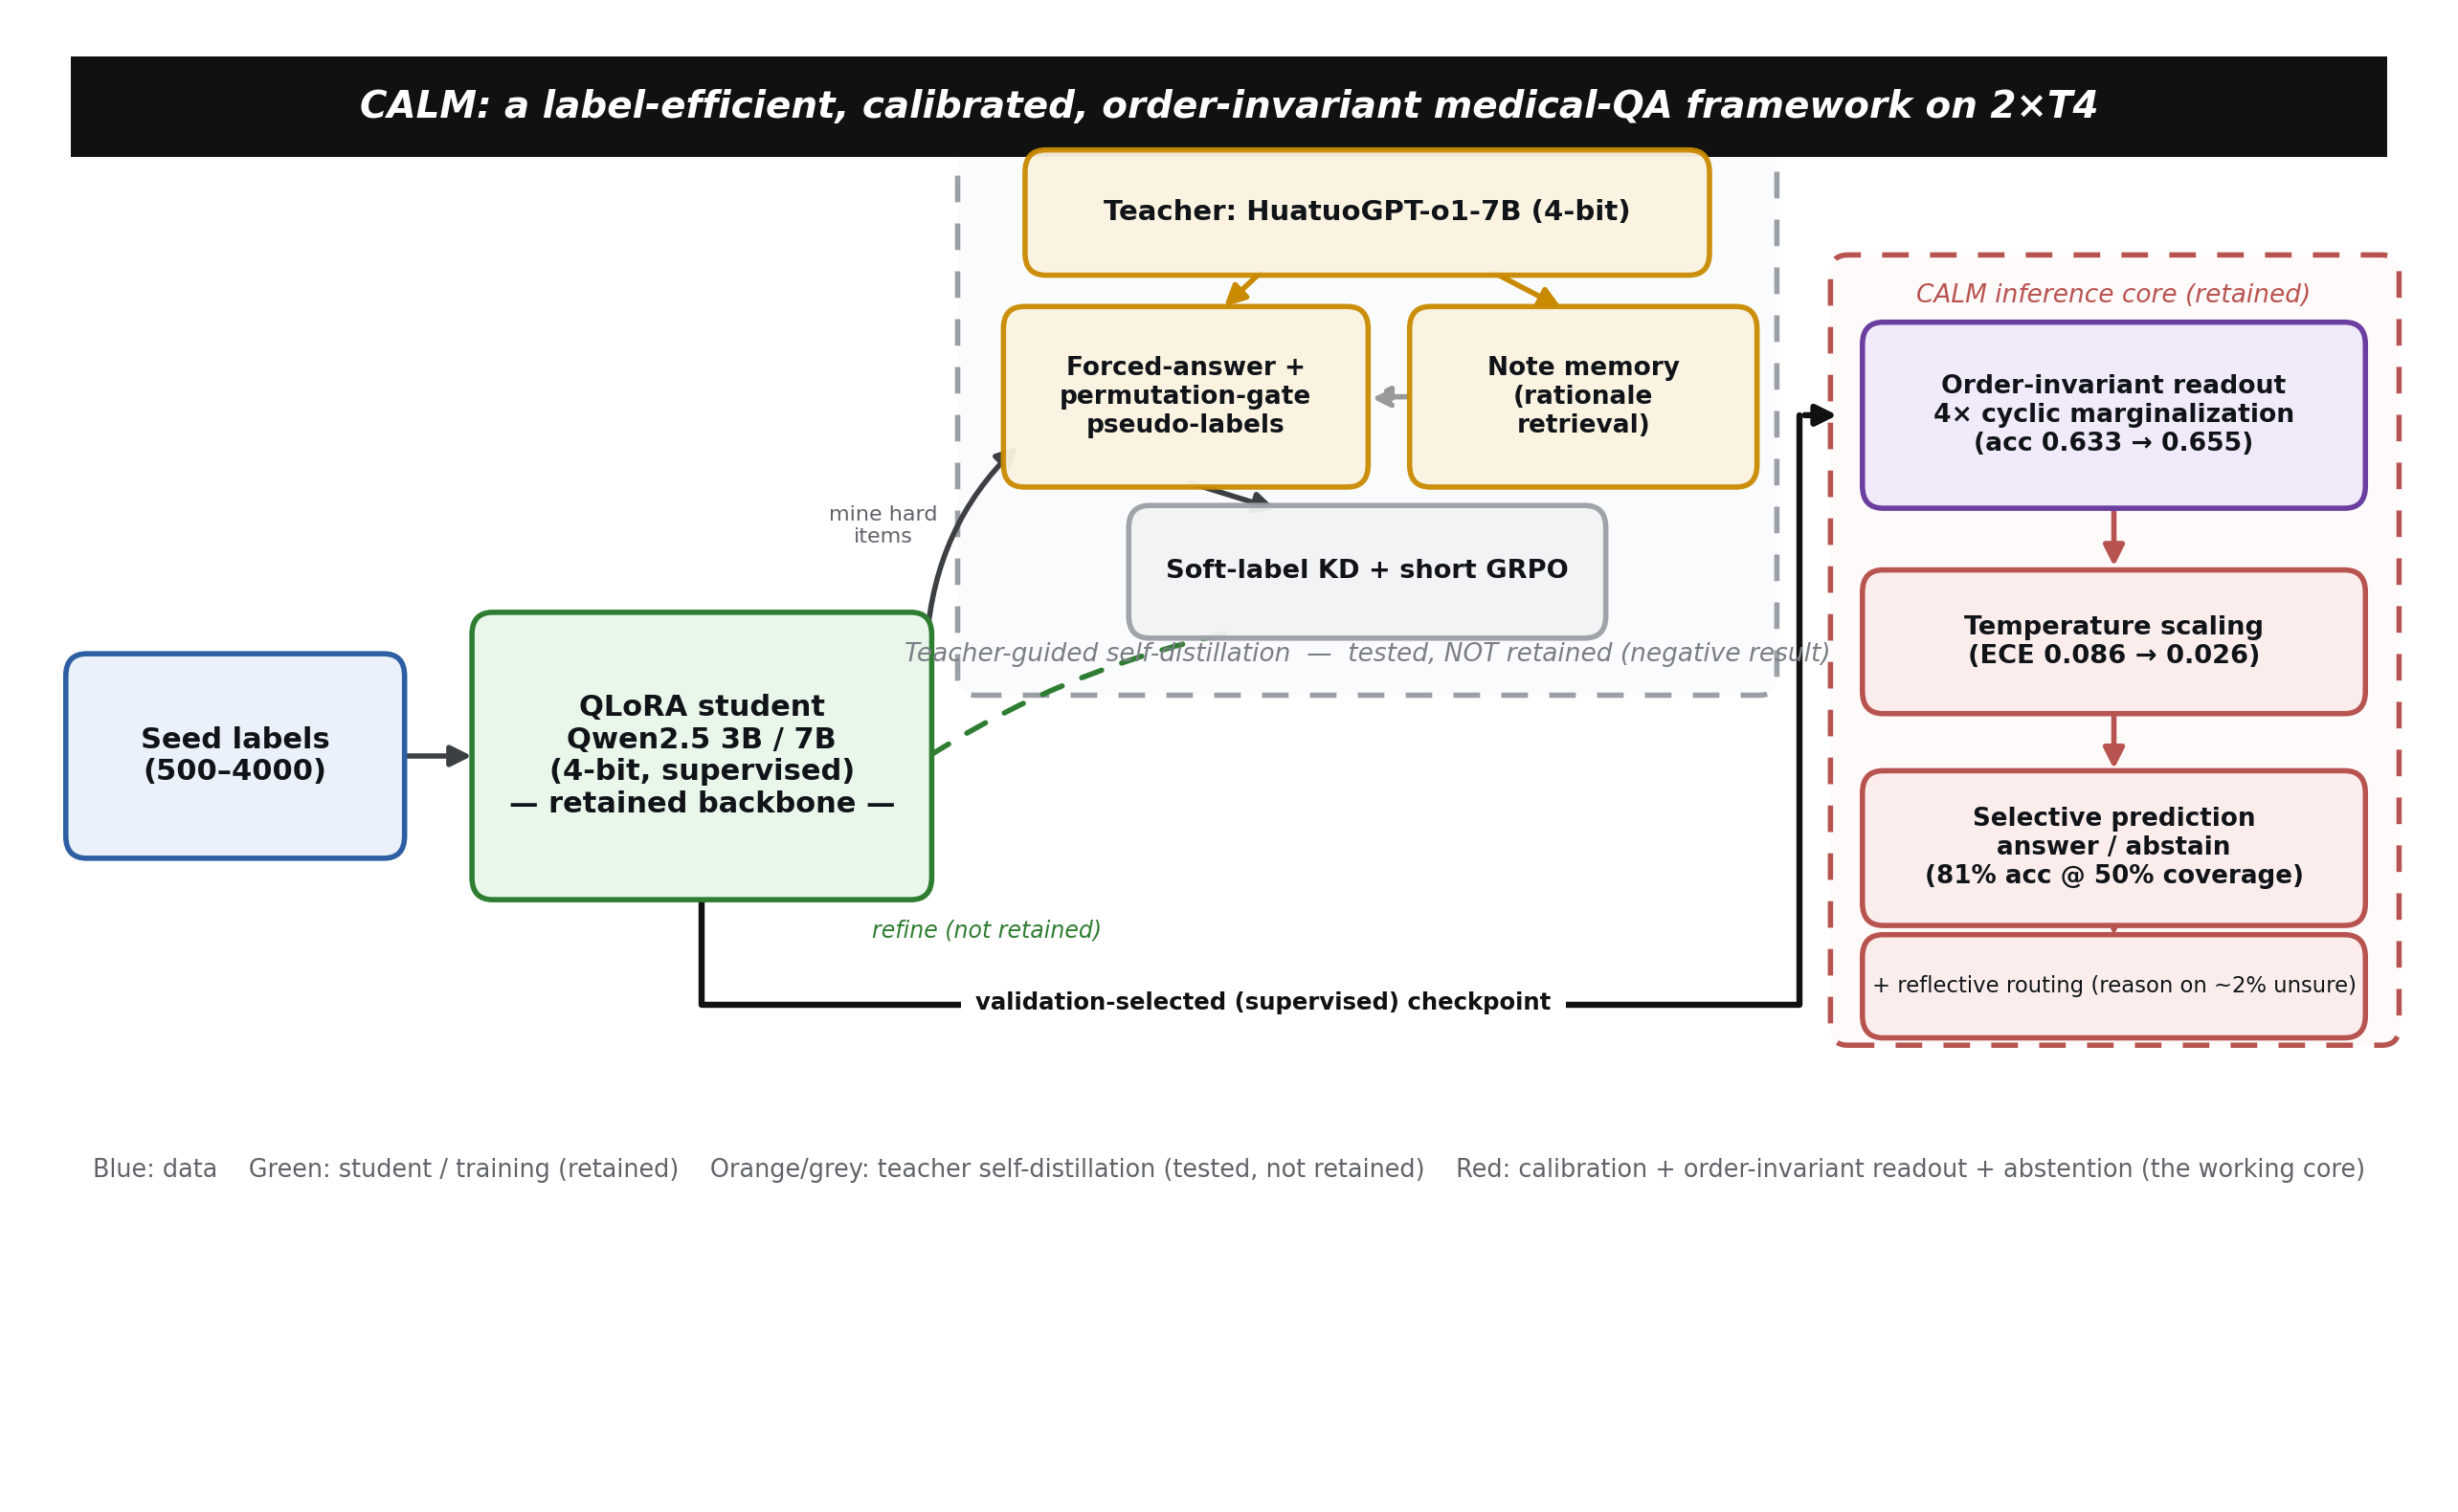
\includegraphics[width=0.95\textwidth]{architecture.png}
\caption{CALM framework. The student is supervised on a small seed set, optionally subjected to the self-distillation stage guided by the teacher, and provided with a post-training calibration and abstention module. Our experiments confirm that the calibration and abstention module adds practical value to the system at this level of budget, while the self-distillation stage does not increase validation accuracy and therefore is not used in the final checkpointing procedure.}\label{fig:arch}
\end{figure*}

\subsection{Setup and student}
Each item consists of a stem $x$, four options, and a letter $y\in\{A,B,C,D\}$. For each dataset, we randomly sample a seed set $\mathcal{D}_{\text{seed}}$ containing 500 to 4{,}000 items and regard the rest of the train split as an unlabeled pool $\mathcal{U}$. The student network is Qwen2.5-3B-Instruct and Qwen2.5-7B-Instruct~\cite{qwen}; we use 4-bit NF4 model with LoRA adaptation on the attention and MLP layers~\cite{lora,qlora}. We evaluate the answer by its next-token logit in the position of the answer. For each option letter $k$, there is a small set of token representations $V_k$ consisting of clean representations without/with leading space; their logit scores are aggregated into $\ell_k=\log\sum_{v\in V_k}\exp z_v$, and normalized as 
\begin{equation}
p_\theta(k\mid x)=\frac{\exp \ell_k}{\sum_{j\in\{A,B,C,D\}}\exp \ell_j}.
\end{equation}
We train on cross-entropy loss for $\mathcal{D}_{\text{seed}}$. The logits are read out by the student without any subsequent reasoning prompt. In the case of selected 7B configuration, the training procedure takes one epoch; in the case of the headline 3B experiment, the training took two epochs and made the model overconfident (Section~\ref{sec:results}); thus, more complicated schedules have not been explored for 7B model.

\subsection{Difficulty mining}
We rank $\mathcal{U}$ using the following score,
\begin{equation}
s(x)=\alpha\,\tilde{H}(x)+(1-\alpha)\bigl(1-\textstyle\max_k p_\theta(k\mid x)\bigr)+\beta\,(1-m(x)),
\end{equation}
where $\tilde{H}(x)$ is the entropy of the distribution over answers (on unnormalized scale with range $[0,\log 4]$), $m(x)=p_{(1)}(x)-p_{(2)}(x)$ is the answer distribution top-two margin, $\alpha=0.5$ and $\beta=0.3$ are the weights on the above scales (this mining $\alpha$ is distinct from the LoRA scaling $\alpha$ in Table~\ref{tab:impl}). Items with maximal scores are sent to the teacher.

\subsection{Two-agreement gates in pseudo-labeling}
A teacher label survives only if two criteria are satisfied: \emph{permutation consistency}, where the teacher is queried on the original option ordering as well as a random permutation, and the choice must be consistent in spite of the re-ordering; and \emph{teacher confidence}, where the maximum probability of an option, calculated via the teacher's first-token softmax over the four letter ids, must be higher than $\gamma=0.55$. The survivors make up $\mathcal{P}$ along with the teacher distribution $p_T$ (the parsed option softmax) as the soft target. Pseudo-label oracle accuracy is not used for training, and is audited only.

\subsection{Note memory, synthesis, and contamination screen}
In addition to writing a rationale in one or two sentences, embedded with all-MiniLM-L6-v2 and saved for nearest neighbor retrieval, teachers discard near-duplicate (cosine $\ge 0.92$) notes. To synthesize neighbors in a subset of hard questions, the teacher re-writes the stem; a neighbor is accepted only if the verifier can derive the same answer. Synthetic near duplicates, with cosine similarity $\ge 0.95$, are filtered out. Contamination screen, which uses no labels and no outcome feedback, is a fixed, pre-specified procedure that filters out every synthetic or pseudo question by comparing it to the test questions using embedding cosine. Since $\mathcal{U}$ is sampled from the training split, no contaminations were detected in either of the runs we report, but the screen is kept as a measure of extra safety.

\subsection{Distillation and reinforcement}
We combine seed cross-entropy with a confidence-weighted distillation term on $\mathcal{P}$. The student's softened distribution is $q_\theta(k\mid x)\propto\exp(\ell_k/T_{\text{KD}})$. The teacher provides parsed option probabilities $p_T$ rather than logits, softened in probability space as $q_T(k\mid x)=p_T(k\mid x)^{1/T_{\text{KD}}}\big/\sum_j p_T(j\mid x)^{1/T_{\text{KD}}}$. Then,
\begin{equation}
\mathcal{L}=\mathbb{E}_{x\sim\mathcal{D}_{\text{seed}}}\!\big[\mathcal{L}_{\text{CE}}\big]
+\lambda\,T_{\text{KD}}^{2}\,\mathbb{E}_{x\sim\mathcal{P}}\!\big[w(x)\,\mathrm{KL}\!\big(q_T\Vert q_\theta\big)\big],
\end{equation}
with distillation temperature $T_{\text{KD}}=3$, distillation weight $\lambda=0.5$, and per-example weight $w(x)=\max_k p_T(k\mid x)$ (the teacher's confidence); the $T_{\text{KD}}^{2}$ factor restores the gradient scale of the softened targets. Then, as in~\cite{grpo}, there follows a short relative-group pass that rewards the student for matching accepted labels through a KL-term with respect to the frozen reference model obtained with the LoRA adapter disabled.

\subsection{Calibration and selective prediction}
Once trained we fit a single calibration temperature $T_{\text{cal}}$ to the validation logits by minimizing NLL~\cite{guocal}, which is independent of the distillation temperature $T_{\text{KD}}$. Confidence is the maximum post-calibrated softmax probability. We measure expected calibration error using ten equal-width bins:
\begin{equation}
\mathrm{ECE}=\sum_{b=1}^{10}\frac{|S_b|}{n}\,\bigl|\,\mathrm{acc}(S_b)-\mathrm{conf}(S_b)\,\bigr|,
\end{equation}
the multiclass Brier score $\frac{1}{n}\sum_i\sum_k {\left[p_{ik}-\mathbf{1}[y_i=k]\right]}^2$, and negative log-likelihood. For selective prediction, we order predictions according to their confidence; at coverage $\tau$ the system predicts the top fraction $\tau$ of instances, with risk $r(\tau)=1-\mathrm{acc}(\tau)$, and we report the summary quantity $\mathrm{AURC}=\int_0^1 r(\tau)\,d\tau$ (trapezoidal on the test set). ``Coverage at 80\% accuracy'' is the maximal $\tau$ such that the accuracy of the top-$\tau$ predictions does not drop below 0.80. These risk-coverage metrics are evaluated on the test split, following the ordering by calibrated confidence; they are not tuned against test labels. We have not selected any operationalization threshold on the test set.

\subsection{Checkpoint selection}\label{sec:selection}
All checkpoints are selected based on their performance on the \emph{validation} split, never the test split. We retain the model that attains the highest validation accuracy. Metrics on the test split and additional diagnostics (label efficiency points, the ablation, the readout comparisons, the shuffle check and contamination tests) that we denote as \emph{post-selection}, rather than model selection. As shown in Section~\ref{sec:results}, the self-distilled checkpoint achieved lower validation accuracy compared to the supervised one for both students; the selection rule retains the supervised model.

\section{Experimental Setup}
Each run is limited to one Kaggle session using two Tesla T4 GPUs (16\,GB each), where the student uses one GPU and the 4-bit teacher the other. The dataset is the MedQA-USMLE four-option multiple-choice question bank. We use a 1{,}000-item validation split (a subset of the official dev set) and the official 1{,}273-item MedQA-USMLE test split; seed and validation sampling use a fixed random seed released with the code. Training uses AdamW with a cosine learning-rate schedule, gradient checkpointing, and only final-token logits, to stay within budget; a wall-clock guard halts the run before the 12-hour session limit. Table~\ref{tab:impl} shows the hyperparameters used for both runs. We measure accuracy, macro-F1, ECE, Brier, NLL, 95\% bootstrap intervals (2{,}000 resamples), the option ordering shuffle test, and the aforementioned abstention metrics. In addition, for the readout and routing comparisons, we compute paired bootstrap intervals of the item-level accuracy difference to determine if the method beats the base reader on the same items. No out-of-memory error occurred on any 16\,GB GPU used.

\begin{table}[tb]
\caption{Implementation details of the two runs that were reported. The cosine row denotes the test-question screening, decontamination of duplicates via note and synthesis, respectively.}\label{tab:impl}
\centering
\scriptsize
\setlength{\tabcolsep}{2pt}
\begin{tabular}{@{}lcc@{}}
\toprule
Setting & 3B run & 7B run \\
\midrule
Student & Qwen2.5-3B-Inst. & Qwen2.5-7B-Inst. \\
Quantization & 4-bit NF4 & 4-bit NF4 \\
LoRA rank/$\alpha$/dropout & 32/64/0.05 & 16/32/0.05 \\
LoRA targets & \multicolumn{2}{c}{q,k,v,o,gate,up,down} \\
Seed labels (headline) & 4000 & 2000 \\
SFT epochs/LR & 2/$1.5\!\times\!10^{-4}$ & 1/$1\!\times\!10^{-4}$ \\
Batch/grad-accum & 8/4 & 4/8 \\
Max source length & 512 & 448 \\
Teacher & \multicolumn{2}{c}{HuatuoGPT-o1-7B (4-bit)} \\
Mining $\alpha,\beta$ & \multicolumn{2}{c}{0.5, 0.3} \\
Pseudo gate $\gamma$ & \multicolumn{2}{c}{0.55} \\
Decontam./note/synth cos. & \multicolumn{2}{c}{0.95/0.92/0.95} \\
KD $T_{\text{KD}},\lambda$, epochs & \multicolumn{2}{c}{3.0, 0.5, 2} \\
GRPO group/LR/KL/epochs & \multicolumn{2}{c}{6/$5\!\times\!10^{-6}$/0.1/1} \\
Embedder & \multicolumn{2}{c}{all-MiniLM-L6-v2} \\
ECE bins & \multicolumn{2}{c}{10 (equal width)} \\
\bottomrule
\end{tabular}
\end{table}

\section{Results}\label{sec:results}

\subsection{Headline numbers}
The results for both models are shown in Table~\ref{tab:main}. The 7B model answers 63.3\% of the test set questions, compared to a 59.2\% zero-shot baseline, and its calibration gain is greater than its accuracy gain, since raw ECE drops from 0.086 to 0.026 with temperature scaling ($T_{\text{cal}}=1.32$). The 3B model answers 52.0\%; for two epochs it had become overconfident (raw ECE 0.36, needed $T_{\text{cal}}=3.6$), but only one epoch of training for the 7B model helped avoid that problem. The 7B headline has a 95\% bootstrap accuracy confidence interval of [0.606, 0.660] and F1 interval of [0.604, 0.657]; accuracy under a random option-order shuffle is 0.631. Calibrated Brier and NLL are 0.48 and 0.89.

\begin{table}[tb]
\caption{Main results on the MedQA-USMLE test split (1{,}273 items). Final = validation-selected checkpoint (Section~\ref{sec:selection}).}\label{tab:main}
\centering
\small
\setlength{\tabcolsep}{3.5pt}
\begin{tabular}{@{}lcccccc@{}}
\toprule
Student & Labels & Zero-shot & Final acc & F1 & ECE$_\text{raw}$ & ECE$_\text{cal}$ \\
\midrule
Qwen2.5-3B & 4000 & 0.481 & 0.520 & 0.517 & 0.356 & 0.046 \\
Qwen2.5-7B & 2000 & 0.592 & \textbf{0.633} & \textbf{0.631} & 0.086 & \textbf{0.026} \\
\bottomrule
\end{tabular}
\end{table}

\subsection{Label efficiency and model scale}
Table~\ref{tab:eff} performs a label-efficiency sweep across the seed size. Each point is a single run, and therefore we view them as observations within the sweep rather than as a general rule. The 7B curve starts rising and then levels off: 500 labels produce 60.1\%, and multiplying by four to 2{,}000 gives an additional 3 points of accuracy while keeping the calibration tightly controlled. The 3B curve is lower and has a wavy shape (0.533, 0.490, 0.522, 0.520), which we explain by overfitting of a small adapter to a small dataset, since in that run the training loss is near zero and a large $T_{\text{cal}}$ is needed. The clear trend lies between the rows: the 7B configuration outperforms the 3B one by roughly 11 points, which is more than the number of labels can help either model.

\begin{table}[tb]
\caption{Label-efficiency sweep (test accuracy; single runs). Calibrated ECE in parentheses for 7B.}\label{tab:eff}
\centering
\small
\setlength{\tabcolsep}{3pt}
\begin{tabular}{@{}lcccc@{}}
\toprule
Student & 500 & 1000 & 2000 & 4000 \\
\midrule
Qwen2.5-3B & 0.533 & 0.490 & 0.522 & 0.520 \\
Qwen2.5-7B & 0.601\,(0.024) & 0.613\,(0.019) & 0.633\,(0.026) & --- \\
\bottomrule
\end{tabular}
\end{table}

\subsection{Calibration and abstention}
In Figure~\ref{fig:reliability}, left side, we present the 7B reliability diagram pre and post calibration. The calibration curve lies close to the diagonal and confidence distinguishes between correct and incorrect answers and can be used in the abstention procedure. From Table~\ref{tab:abstain} and Figure~\ref{fig:reliability} (right), one can see that the behavior of the abstention is as follows: on this test split, at 50\% coverage the 7B reader is correct 80.8\% of the time, and on the test risk--coverage curve the most-confident $\approx$51\% are answered at $\ge$80\% accuracy (cov@80 $=0.513$, a curve summary rather than a deployed threshold). This is how the selective prediction results look for this test split. Single-split point estimates of per-coverage accuracy intervals are presented below; per-coverage accuracy intervals bootstrap will be done in the future. There is no collapse into one option for the errors but all the four options are equally represented – consistent with the shuffle check.

\begin{table}[tb]
\caption{Selective prediction on the test split: risk--coverage summaries from the calibrated-confidence ranking {not a threshold tuned on test}. Here acc@$c$ is accuracy on the most-confident $c\%$ of test items; cov@80 is the largest coverage whose answered accuracy stays $\ge$0.80; AURC is the area under the risk--coverage curve (lower is better). Point estimates.}\label{tab:abstain}
\centering
\small
\setlength{\tabcolsep}{4pt}
\begin{tabular}{@{}lccccc@{}}
\toprule
Student & acc@50 & acc@70 & acc@90 & AURC & cov@80 \\
\midrule
Qwen2.5-3B & 0.668 & 0.608 & 0.548 & 0.321 & 0.144 \\
Qwen2.5-7B & \textbf{0.808} & \textbf{0.737} & \textbf{0.668} & \textbf{0.185} & \textbf{0.513} \\
\bottomrule
\end{tabular}
\end{table}

\begin{figure*}[t]
\centering
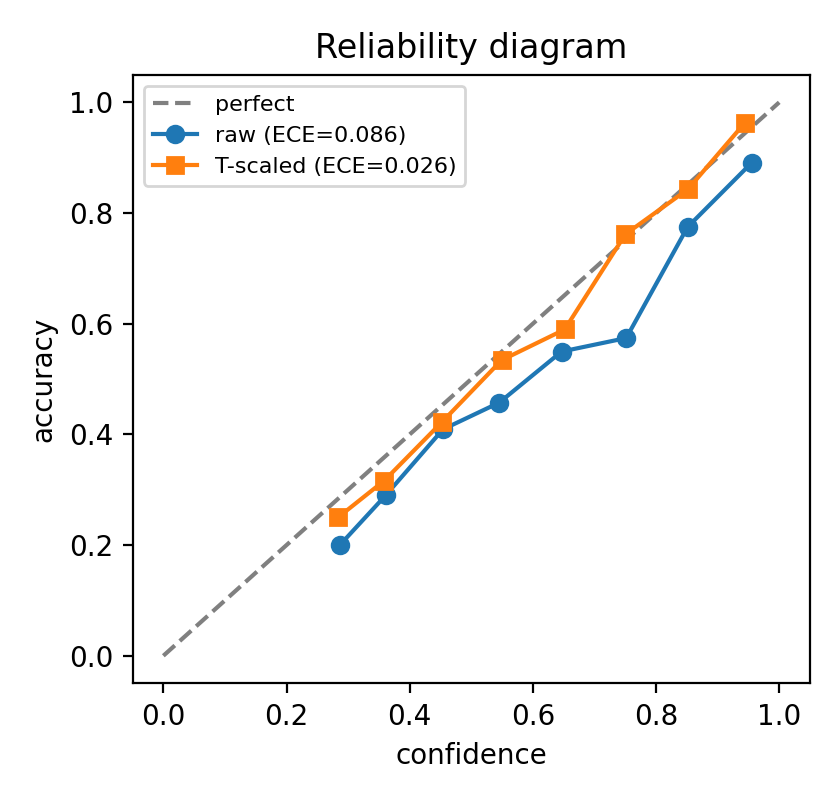
\includegraphics[height=5cm]{reliability_combined.png}\hspace{0.05\textwidth}
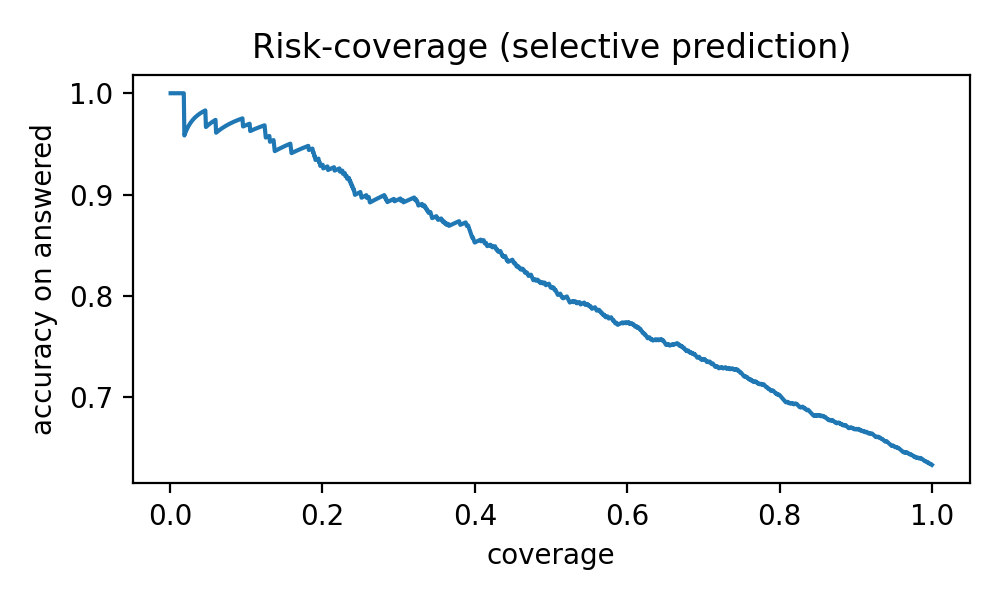
\includegraphics[height=5cm]{risk_coverage.png}
\caption{Calibration and selective prediction for the 7B student. Left panel: reliability diagram before and after temperature scaling (ECE $0.086\!\to\!0.026$); the calibrated curve remains close to the ideal diagonal. Right panel: risk--coverage behavior; selecting the most confident half of the predictions increases accuracy from 63\% to about 81\%.}\label{fig:reliability}
\end{figure*}

\subsection{An order-invariant readout}\label{sec:pi}
A multiple-choice reader will sometimes revise its decision on the question as the four options are shuffled~\cite{robustmcq,permbias}. Our 7B student is slightly prone to doing so, as the accuracy ranges from 0.623 to 0.651 in its four cyclic shifts. We will now use that fact to our advantage. On each question, we run the four cyclic shifts of the option block, where each letter appears exactly once, compute the per-content probability from each shift, and average
\begin{equation}
\bar{p}(c\mid x)=\frac{1}{4}\sum_{s=0}^{3}
p_\theta\!\big(d=(c-s)\bmod 4 \;\big|\; x,\pi_s\big),
\end{equation}
where displayed letters are indexed $d\in\{0,1,2,3\}$ for A--D, and $\pi_s$ is the cyclic shift by $s$ that places option content $c$ at displayed position $(c-s)\bmod 4$ (we keep $\ell_k$ for the aggregated option logit of the setup). We then fit a calibration temperature for this reader on the validation split, with the same NLL objective as the base reader; it comes out to $T=1.15$ (versus $T=1.32$ for the base reader). Fitting this single scalar uses the existing validation split---no new labels and no model training---and the four-pass readout itself decodes nothing.

In Table~\ref{tab:pi}, we show the effects of the procedure on the full test split with bootstrap intervals. The marginalization increases accuracy from 0.633 to 0.655, a paired gain of $+0.022$ with 95\% CI $[+0.006,+0.038]$, and enhances selective prediction (AURC $0.185\!\to\!0.177$, Brier $0.480\!\to\!0.469$). The confidence intervals of the marginal and base reader accuracies do overlap; however, the paired interval, which shows the difference between the two on the same set of questions, proves the gain. A reasonable baseline---removing the option ID prior like in PriDe~\cite{robustmcq}---does nothing in our case ($+0.000$, CI $[-0.018,+0.018]$)---the estimated prior was almost uniform, $[0.25,0.25,0.26,0.24]$, so there was no letter bias to correct. Why help at all if there is no prior to remove? Variance. The four orderings disagree on some items, and averaging them is a tiny self-ensemble---which is exactly why the marginalized reader (0.655) edges out even the best single ordering (0.651). The calibration remains excellent (ECE 0.032). The base ECE in Table~\ref{tab:pi} (0.024) is marginally lower than in Table~\ref{tab:main} (0.026) because this run refits the temperature on a 500-item validation subset; the checkpoint is identical and the gap is within the run-to-run variation of the scalar fit. In Figure~\ref{fig:pi}, we show the risk--coverage curve of the marginalized reader being lower than that of the base reader at all coverages.

\begin{table}[tb]
\caption{Readouts on the full MedQA-USMLE test split (1{,}273 items), all temperature-calibrated. The passes column indicates how many forward passes per question are done; none decode tokens. $\Delta$acc is the paired accuracy gain of the readout over the base reader with 95\% bootstrap CI.}\label{tab:pi}
\centering
\footnotesize
\setlength{\tabcolsep}{2pt}
\begin{tabular}{@{}lccccc@{}}
\toprule
Readout & passes & acc & ECE & AURC & $\Delta$acc \\
\midrule
Base (calibrated)        & 1 & 0.633 & 0.024 & 0.185 & --- \\
PriDe~\cite{robustmcq}   & 1 & 0.633 & 0.041 & 0.188 & $+0.000$ $[-0.018,+0.018]$ \\
\textbf{Cyclic-marg.} & 4 & \textbf{0.655} & 0.032 & \textbf{0.177} & $\mathbf{+0.022}$ $[+0.006,+0.038]$ \\
\bottomrule
\end{tabular}
\end{table}

\begin{figure}[tb]
\centering
\includegraphics[width=\linewidth]{pi_risk_coverage.png}
\caption{Risk--coverage comparison on the test split between the base calibrated reader and the order-invariant (cyclic-marginalized) reader. The marginalized version obtains lower risk across all coverage levels, improving both accuracy and selective prediction.}\label{fig:pi}
\end{figure}

\subsection{Selective reasoning and reflective routing}\label{sec:r3}
Reasoning does not seem to be useful for this student in general. Even on a smaller 134-question matched subset (Table~\ref{tab:sc}), a single calibrated reasoning pass beats the five-sample self-consistency in both accuracy (0.709 vs 0.493) and selective prediction (AURC 0.128 vs 0.289), spending a much smaller decoding budget: a single forward pass reading the logits of four options against five samples, each of up to 256 tokens long. One reason is probably the degradation of chain-of-thought skills due to fine-tuning of the student as a one-pass answerer.

That leads us to the next, more specific question: does reasoning help in the \emph{uncertain cases}, where the model does not have enough evidence to confidently make an inference? The selection policy is calibrated confidence-based, meaning answering with the fast logit read when the top option has a high confidence, and sending the questions requiring reasoning to a single reasoning pass---the confidence threshold is chosen during validation. Table~\ref{tab:r3} demonstrates the effect on the full test set split. Routing just the 2\% most uncertain items increases accuracy from 0.633 to 0.639, gaining $+0.006$ paired with 95\% bootstrap confidence interval of $[+0.002,+0.012]$. The additional decoding overhead per question is about 2 tokens on average, over the entire split. This is a marginal adaptive computing gain, and it is achieved without any additional training: training a reflect adapter on the hard subset with reflective correction loss---cross-entropy for the wrong fast answer, consistency with the confident fast answer---performs no better than the base student's own reasoning ($+0.002$, CI $[-0.002,+0.008]$), consistent with overfitting a few hundred hard items. We did not stack routing on top of the order-invariant reader; the two are separate inference-time options, and a combined system is left to future work.

\begin{table}[tb]
\caption{Reflective routing on the full test split. $\Delta$acc is the gain over the fast-only reader with 95\% bootstrap confidence interval; tokens/q is decoded tokens per question averaged over the split.}\label{tab:r3}
\centering
\footnotesize
\setlength{\tabcolsep}{2pt}
\begin{tabular}{@{}lcccc@{}}
\toprule
Policy & acc & $\Delta$acc & \% reas. & tokens/q \\
\midrule
Fast-only & 0.633 & --- & 0 & 0 \\
\textbf{Routed (untrained)} & \textbf{0.639} & $\mathbf{+0.006}$ $[+0.002,+0.012]$ & 2 & 2.2 \\
Routed (trained) & 0.636 & $+0.002$ $[-0.002,+0.008]$ & 2 & 2.0 \\
\bottomrule
\end{tabular}
\end{table}

\begin{table}[tb]
\caption{Single calibrated pass vs.\ self-consistency reasoning (7B, matched 134-item subset).}\label{tab:sc}
\centering
\small
\setlength{\tabcolsep}{4pt}
\begin{tabular}{@{}lccc@{}}
\toprule
Method & Acc & AURC & samples $\times$ gen tokens \\
\midrule
Single calibrated pass & \textbf{0.709} & \textbf{0.128} & $1\times1$ (logit read) \\
Self-consistency CoT & 0.493 & 0.289 & $5\times{\le}256$ \\
\bottomrule
\end{tabular}
\end{table}

\subsection{Design analysis: the self-distillation stage}
Table~\ref{tab:abl} shows that the self-distillation stage decreases the \emph{validation} accuracy of the students---from 0.637 to 0.614 for 7B, from 0.514 to 0.507 for 3B---and the test accuracy follows (for 7B: 0.633$\to$0.614; 3B: 0.520$\to$0.517). Thus, the validation-based rule of Section~\ref{sec:selection} retains the supervised checkpoint, and the headline results are the scores of the supervised model. The reason is clear from the logs: the teacher accepts just several dozen labels in the hard items with an oracle accuracy of around 0.46--0.66 while there are thousands of clean labels used as seeds---not enough, inaccurate, and concentrated on the questions which are most uncertain for both the teacher and the student. Thus, we report this result as negative: with this budget, the self-distillation stage of CALM does not improve the performance. The pipeline audit (Table~\ref{tab:audit}) shows the extent: for the 7B run, the gates reject 150 mined questions down to 79 consistent and 68 passing the confidence gate, 80 synthetic questions were accepted and 35 were rejected, and the test question screening rejects none.

\begin{table}[tb]
\caption{Self-distillation ablation. Validation accuracy dictates the choice of the checkpoint; test accuracy is reported for reference. The stage is discarded.}\label{tab:abl}
\centering
\small
\setlength{\tabcolsep}{3.5pt}
\begin{tabular}{@{}lcccc@{}}
\toprule
 & \multicolumn{2}{c}{Val acc} & \multicolumn{2}{c}{Test acc} \\
Student & SFT & +self-dist. & SFT & +self-dist. \\
\midrule
Qwen2.5-3B & \textbf{0.514} & 0.507 & 0.520 & 0.517 \\
Qwen2.5-7B & \textbf{0.637} & 0.614 & 0.633 & 0.614 \\
\bottomrule
\end{tabular}
\end{table}

\begin{table}[tb]
\caption{Pseudo-labeling and synthesis audit (one iteration). The columns show the number of items passed to the teacher, the number of pseudo-labels accepted after gates, the accuracy of the pseudo-labels with respect to the ground truth, the number of synthetic items kept, the number of synthetic items rejected, and the number of items rejected by the test-question screening; ``---'' denotes the counts that were not logged for the 3B run.}\label{tab:audit}
\centering
\footnotesize
\setlength{\tabcolsep}{3pt}
\begin{tabular}{@{}lcccccc@{}}
\toprule
Run & mined & accept. & PAcc & synth kept & synth rej. & decon. \\
\midrule
3B (4000) & 150 & 79 & 0.658 & --- & --- & 0 \\
7B (2000) & 150 & 68 & 0.456 & 80 & 35 & 0 \\
\bottomrule
\end{tabular}
\end{table}

\subsection{Context}
Table~\ref{tab:context} shows our numbers compared to larger-scale systems. All the values are taken from the cited papers as reported there within their settings and are not directly comparable; we present them only to specify the operating regime. A 7B model fine-tuned from 2{,}000 labels on two free T4s is sufficiently accurate and, unlike the raw base, offers calibrated confidence, an abstention strategy, and an order-invariant output.

\begin{table}[tb]
\caption{Context only. Values are as reported (rounded) by the cited sources under their own settings and are not directly comparable. The Qwen2.5-7B row is the zero-shot value reported by~\cite{qwen}; under our own prompt and evaluation the same base scores 0.592 (Table~\ref{tab:main}).}\label{tab:context}
\centering
\small
\setlength{\tabcolsep}{3pt}
\begin{tabular}{@{}lccc@{}}
\toprule
System & Size & MedQA & Setting \\
\midrule
GPT-4~\cite{gpt4med} & undisclosed & $\approx$0.86 & prompting \\
Med-PaLM~2~\cite{medpalm} & undisclosed & $\approx$0.86 & full-data \\
Meerkat~\cite{meerkat} & 7B & 0.77 & reasoning-data \\
MedMobile~\cite{medmobile} & 3.8B & 0.76 & full-data \\
Qwen2.5-7B~\cite{qwen} & 7B & $\approx$0.51 & zero-shot \\
\textbf{Ours (7B, 2k labels)} & 7B & \textbf{0.655} & this work \\
\bottomrule
\end{tabular}
\end{table}

\section{Discussion}
The biggest surprise was the option-order experiment. We added it mainly as a robustness check, and it turned into the largest inference-time gain we found. The base configuration still mattered most: the 7B run beat the 3B run by more than any label count moved either of them, and once the base was fixed a few hundred labels already flattened the curve. (The two runs differ in more than parameter count, so we are not isolating scale.) Calibration came next; one temperature made the confidence worth acting on, which is what abstention and routing both rely on. Reasoning helped only in small, targeted doses, and a reflect adapter trained for it helped not at all. The two additions we most expected to pay off---self-distillation and self-consistency---did not: the first lowered validation accuracy, the second lost to a single calibrated pass on the matched 134-item subset.

These measurements allow us to keep CALM lean: the selected by our validation routine configuration consists of supervised adaptation with calibration, abstention, and an order-invariant readout; the teacher-guided stage and the reasoning adapter are included among the tested configurations only. This is the advice we can give regarding small medical-QA models on commodity hardware.

\section{Limitations}
This paper evaluates one English benchmark on one test split, with single runs of sweep parameters versus averages of multiple seeds, hence the observed trends cannot be considered as universal laws. While the accuracy ($\approx$0.65) falls significantly short of specialist models fine-tuned on the full dataset, the order-invariant readout entails four forward passes per question (no decoding involved yet). The routing boost is also relatively minor and relies on only a small percent of the questions. Calibration and abstention are measured in a post-hoc way on the benchmark split; this does not imply robustness in terms of distribution shift, prospective calibration, or any kind of clinical workflow validation; we make no claim on deployment. The contamination screen against test questions is a deterministic label-free audit, but the very use of the test inputs as a sensitivity measure is notable. The comparison of costs of self-consistency versus decoding is a theoretical argument, not a benchmark on wall clock time.

\section{Conclusion}
Two T4s, several thousands of labeled examples, quantized adapters. In those conditions, a Qwen2.5-7B QLoRA student achieves 0.633 accuracy on the MedQA-USMLE test split and calibrated to an ECE of 0.026 with just one parameter; its top half makes predictions at 80\% accuracy. A training-free order-invariant readout raises the test accuracy to 0.655 and lowers risk--coverage; separately, confidence-gated routing gives a small, significant gain over the fast reader at negligible overhead (we did not measure it on top of the order-invariant reader). We have tried to state plainly what helped and what did not: a stronger base, calibration, and order averaging helped; teacher-guided self-distillation, self-consistency (on a matched subset), and training a reflect adapter did not. The final system is not complicated. In our experiments most of the benefit came from the base-model choice, calibration, and reducing option-order variance.

\section*{Reproducibility}
All training and evaluation code, configuration files, prompts, splits definitions, exported metric artifacts and figures will be released after publication in order to reproduce the reported numbers on the same two-T4 configuration.

\section*{Acknowledgment}
The authors would like to thank the open-source community and Kaggle for providing access to T4 hardware. A generative AI assistant was used for language editing of the manuscript; however, all experiments, analysis, and conclusions belong to the authors exclusively.
\begin{thebibliography}{00}
\bibitem{medqa} D. Jin, E. Pan, N. Oufattole, W.-H. Weng, H. Fang, and P. Szolovits, ``What disease does this patient have? A large-scale open domain question answering dataset from medical exams'', \emph{Applied Sciences}, vol.~11, no.~14, 2021.
\bibitem{gpt4med} H. Nori, N. King, S. M. McKinney, D. Carignan, and E. Horvitz, ``Capabilities of GPT-4 on medical challenge problems'', arXiv:2303.13375, 2023.
\bibitem{medpalm} K. Singhal \emph{et al.}, ``Towards expert-level medical question answering with large language models'', \emph{Nature Medicine}, 2025.
\bibitem{meerkat} H. Kim \emph{et al.}, ``Small language models learn enhanced reasoning skills from medical textbooks'', \emph{npj Digital Medicine}, 2025.
\bibitem{medmobile} K. Vishwanath \emph{et al.}, ``MedMobile: A mobile-sized language model with clinical capabilities'', arXiv:2410.09019, 2024.
\bibitem{huatuo} J. Chen \emph{et al.}, ``HuatuoGPT-o1: Towards medical complex reasoning with LLMs'', arXiv:2412.18925, 2024.
\bibitem{hinton} G. Hinton, O. Vinyals, and J. Dean, ``Distilling the knowledge in a neural network'', arXiv:1503.02531, 2015.
\bibitem{star} E.~Zelikman, Y. Wu, J. Mu, and N. Goodman, ``STaR\@: Bootstrapping reasoning with reasoning'', in \emph{NeurIPS}, 2022.
\bibitem{selfconsistency} X. Wang \emph{et al.}, ``Self-consistency improves chain of thought reasoning in language models'', in \emph{ICLR}, 2023.
\bibitem{pseudolabel} D.-H. Lee, ``Pseudo-label: The simple and efficient semi-supervised learning method for deep neural networks'', in \emph{ICML Workshop}, 2013.
\bibitem{lora} E.~J.~Hu \emph{et al.}, ``LoRA\@: Low-rank adaptation of large language models'', in \emph{ICLR}, 2022.
\bibitem{qlora} T.~Dettmers, A. Pagnoni, A. Holtzman, and L. Zettlemoyer, ``QLoRA\@: Efficient finetuning of quantized LLMs'', in \emph{NeurIPS}, 2023.
\bibitem{guocal} C. Guo, G. Pleiss, Y. Sun, and K. Q. Weinberger, ``On calibration of modern neural networks'', in \emph{ICML}, 2017.
\bibitem{selectivenet} Y. Geifman and R. El-Yaniv, ``SelectiveNet: A deep neural network with an integrated reject option'', in \emph{ICML}, 2019.
\bibitem{abstain} H. Wen \emph{et al.}, ``Know your limits: A survey of abstention in large language models'', \emph{Transactions of the Association for Computational Linguistics}, 2025.
\bibitem{trustsurvey} Y. Wang, R. E. Mercer, F. Rudzicz \emph{et al.}, ``Trustworthy medical question answering: An evaluation-centric survey'', arXiv:2506.03659, 2025.
\bibitem{robustmcq} C. Zheng, H. Zhou, F. Meng, J. Zhou, and M. Huang, ``Large language models are not robust multiple choice selectors'', in \emph{Proc. ICLR}, 2024.
\bibitem{permbias} Y. Zong, T. Yu, R. Chavhan, B. Zhao, and T. Hospedales, ``Fool your (vision and) language model with embarrassingly simple permutations'', in \emph{Proc. ICML}, 2024.
\bibitem{grpo} Z. Shao \emph{et al.}, ``DeepSeekMath: Pushing the limits of mathematical reasoning in open language models'', arXiv:2402.03300, 2024.
\bibitem{smallrl} Q. Dao \emph{et al.}, ``Reinforcement learning for reasoning in small LLMs: What works and what doesn't'', arXiv:2503.16219, 2025.
\bibitem{qwen} A. Yang \emph{et al.}, ``Qwen2.5 technical report'', arXiv:2412.15115, 2024.
\end{thebibliography}

\end{document}
